\documentclass[10pt,a4paper,oneside,abstracton]{scrartcl}
\usepackage[utf8]{inputenc}
\usepackage[english, ngerman]{babel}

\usepackage{amsmath}
\usepackage{amsfonts}
\usepackage{amssymb}
\usepackage{graphicx}
\usepackage{lmodern}
	%\usepackage{kpfonts}
\usepackage{fourier}
\usepackage[left=2cm,right=2cm,top=2cm,bottom=2cm]{geometry}
\usepackage{multicol}
\setcounter{secnumdepth}{4} %Nummerierungstiefe bis Paragraph (4. Ebene)
\usepackage{blindtext}
\usepackage[ 		%Einstellungen für Link
   colorlinks,        % Link ohne Umrandungen in zu wählender Farbe 
   linkcolor=black,   % Farbe interner Verweise 
   filecolor=black,   % Farbe externer Verweise 
   citecolor=black    % Farbe von Zitaten 
]{hyperref}
\pagestyle{empty}		%Seitenzahl wird nich angezeigt

\begin{document}

\section*{Beitragstitel}
\section*{Title of contribution}
Titel, Vorname und Nachname des/der Autors/Autoren, Firma/Institution, Ort, Land, e-Mail(10/12pt) 


\begin{abstract} %kann man auch ueber /subsection machen
\noindent %einrücken verhindern
Dies ist ein normaler Text in 10 pt Schriftgröße und 12 pt Zeilenabstand. Dies ist ein normaler Text in 10 pt Schriftgröße und 12 pt Zeilenabstand. Dies ist ein normaler Text in 10 pt Schriftgröße und 12 pt Zeilenabstand. Dies ist ein normaler Text in 10 pt Schriftgröße und 12 pt Zeilenabstand. Dies ist ein normaler Text in 10 pt Schriftgröße und 12 pt Zeilenab-stand. Dies ist ein normaler Text in 10 pt Schriftgröße und 12 pt Zeilenabstand. Dies ist ein normaler Text in 10 pt Schriftgröße und 12 pt Zeilenabstand. Dies ist ein normaler Text in 10 pt Schriftgröße und 12 pt Zeilenabstand. Dies ist ein normaler Text in 10 pt Schriftgröße und 12 pt Zeilenabstand.
\end{abstract}

\renewcommand{\abstractname}{Abstract} %aendert name Zusammenfassung in Abstract

\begin{abstract}
\noindent %einrücken verhindern
Dies ist ein normaler Text in 10 pt Schriftgröße und 12 pt Zeilenabstand. Dies ist ein normaler Text in 10 pt Schrift-größe und 12 pt Zeilenabstand. Dies ist ein normaler Text in 10 pt Schriftgröße und 12 pt Zeilenabstand. Dies ist ein normaler Text in 10 pt Schriftgröße und 12 pt Zeilen-abstand. Dies ist ein normaler Text in 10 pt Schriftgröße und 12 pt Zeilenabstand.
\end{abstract}


\begin{multicols}{2}
\section{Dies ist eine Überschrift 1. Ordnung}
Dies ist ein normaler Text in 10 pt Schriftgröße und 12 pt Zeilenabstand. Dies ist ein normaler Text in 10 pt Schrift-größe und 12 pt Zeilenabstand. Dies ist ein normaler Text in 10 pt Schriftgröße und 12 pt Zeilenabstand. Dies ist ein normaler Text in 10 pt Schriftgröße und 12 pt Zeilen-abstand. Dies ist ein Dies ist ein normaler Text in 10 pt Schriftgröße und 12 pt Zeilenabstand.


\subsection{Dies ist eine Überschrift 2. Ordnung}
Dies ist ein normaler Text in 10 pt Schrift-größe und 12 pt Zeilenabstand. Dies ist ein normaler Text in 10 pt Schriftgröße und 12 pt Zeilenabstand.
 Dies ist ein normaler Text in 10 pt Schriftgröße und 12 pt Zeilen-abstand. Dies ist ein normaler Text in 10 pt Schriftgröße und 12 pt Zeilenabstand.normaler Text in 10 pt Schriftgröße und 12 pt Zeilenabstand. Dies ist ein normaler Text in 10 pt Schrift-größe und 12 pt Zeilenabstand. Dies ist ein normaler Text in 10 pt Schriftgröße und 12 pt Zeilenabstand. Dies ist ein normaler Text in 10 pt Schriftgröße und 12 pt Zeilen-abstand. Dies ist ein normaler Text in 10 pt Schriftgröße und 12 pt Zeilenabstand.normaler Text in 10 pt Schriftgröße und 12 pt Zeilenabstand.
%\vfill				%Genaue Abtrennung nach diesem Wort
%\columnbreak 		%Beginnt neue spalte
Dies ist ein normaler Text in 10 pt Schrift-größe und 12 pt Zeilenabstand. Dies ist ein normaler Text in 10 pt Schriftgröße und 12 pt Zeilenabstand.
 Dies ist ein normaler Text in 10 pt Schriftgröße und 12 pt Zeilen-abstand. Dies ist ein normaler Text in 10 pt Schriftgröße und 12 pt Zeilenabstand.normaler Text in 10 pt Schriftgröße und 12 pt Zeilenabstand. Dies ist ein normaler Text in 10 pt Schrift-größe und 12 pt Zeilenabstand. Dies ist ein normaler Text in 10 pt Schriftgröße und 12 pt Zeilenabstand.

\subsubsection{Dies ist eine Überschrift 3. Ordnung}

 Dies ist ein normaler Text in 10 pt Schriftgröße und 12 pt Zeilen-abstand. Dies ist ein normaler Text in 10 pt Schriftgröße und 12 pt Zeilenabstand.normaler Text in 10 pt Schriftgröße und 12 pt Zeilenabstand. Dies ist ein normaler Text in 10 pt Schrift-größe und 12 pt Zeilenabstand. Dies ist ein normaler Text in 10 pt Schriftgröße und 12 pt Zeilenabstand.
 Dies ist ein normaler Text in 10 pt Schriftgröße und 12 pt Zeilen-abstand. Dies ist ein normaler Text in 10 pt Schriftgröße und 12 pt Zeilenabstand.normaler Text in 10 pt Schriftgröße und 12 pt Zeilenabstand. Dies ist ein normaler Text in 10 pt Schrift-größe und 12 pt Zeilenabstand. Dies ist ein normaler Text in 10 pt Schriftgröße und 12 pt Zeilenabstand.
 Dies ist ein normaler Text in 10 pt Schriftgröße und 12 pt Zeilen-abstand. Dies ist ein normaler Text in 10 pt Schriftgröße und 12 pt Zeilenabstand.normaler Text in 10 pt Schriftgröße und 12 pt Zeilenabstand. Dies ist ein normaler Text in 10 pt Schrift-größe und 12 pt Zeilenabstand. Dies ist ein normaler Text in 10 pt Schriftgröße und 12 pt Zeilenabstand.
 Dies ist ein normaler Text in 10 pt Schriftgröße und 12 pt Zeilen-abstand. Dies ist ein normaler Text in 10 pt Schriftgröße und 12 pt Zeilenabstand.normaler Text in 10 pt Schriftgröße und 12 pt Zeilenabstand. Dies ist ein normaler Text in 10 pt Schrift-größe und 12 pt Zeilenabstand. Dies ist ein normaler Text in 10 pt Schriftgröße und 12 pt Zeilenabstand.
 Dies ist ein normaler Text in 10 pt Schriftgröße und 12 pt Zeilen-abstand. Dies ist ein normaler Text in 10 pt Schriftgröße und 12 pt Zeilenabstand.normaler Text in 10 pt Schriftgröße und 12 pt Zeilenabstand. Dies ist ein normaler Text in 10 pt Schrift-größe und 12 pt Zeilenabstand. Dies ist ein normaler Text in 10 pt Schriftgröße und 12 pt Zeilenabstand.
 Dies ist ein normaler Text in 10 pt Schriftgröße und 12 pt Zeilen-abstand. Dies ist ein normaler Text in 10 pt Schriftgröße und 12 pt Zeilenabstand.normaler Text in 10 pt Schriftgröße und 12 pt Zeilenabstand. 


$\rho = \frac{m}{V}$

\begin{equation}
{\rho = \frac{m}{V}}
\end{equation}

Dies ist ein normaler Text in 10 pt Schrift-größe und 12 pt Zeilenabstand. Dies ist ein normaler Text in 10 pt Schriftgröße und 12 pt Zeilenabstand.
 Dies ist ein normaler Text in 10 pt Schriftgröße und 12 pt Zeilen-abstand. Dies ist ein normaler Text in 10 pt Schriftgröße und 12 pt Zeilenabstand.normaler Text in 10 pt Schriftgröße und 12 pt Zeilenabstand. Dies ist ein normaler Text in 10 pt Schrift-größe und 12 pt Zeilenabstand. Dies ist ein normaler Text in 10 pt Schriftgröße und 12 pt Zeilenabstand. 
 
\paragraph{Dies ist eine Überschrift 4. Ordnung} $\;$\\%Trick zu Erzeugung eines Zeilenumbruchs
Dies ist ein normaler Text in 10 pt Schriftgröße und 12 pt Zeilen-abstand. Dies ist ein normaler Text in 10 pt Schriftgröße und 12 pt Zeilenabstand.normaler Text in 10 pt Schriftgröße und 12 pt Zeilenabstand.Dies ist ein normaler Text in 10 pt Schriftgröße und 12 pt Zeilenabstandnormaler Text in 10 pt Schriftgröße und 12 pt Zeilenabstand.
	
	
\noindent%
\begin{minipage}{0.9\columnwidth}  %.9 auf 90 Prozent skaliert 
\centering 
\resizebox{0.9\columnwidth}{!} 
{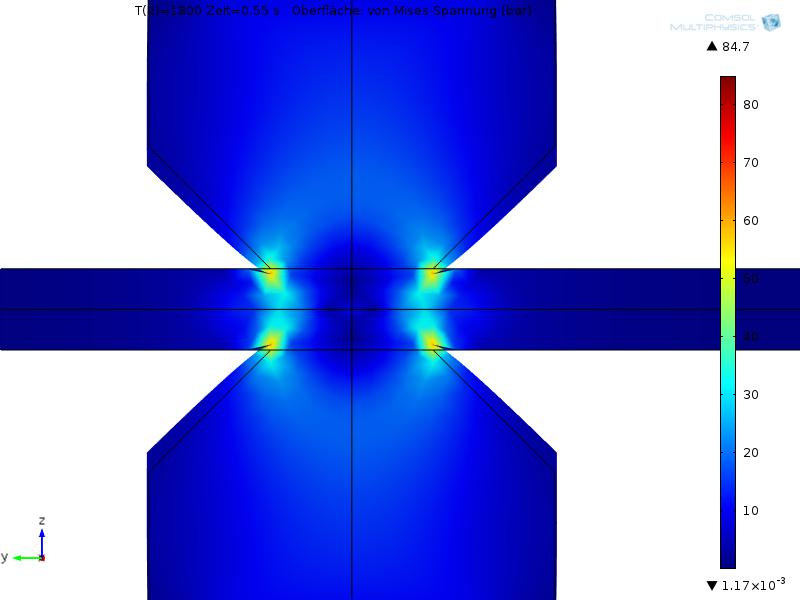
\includegraphics[width=\textwidth]{./Bilder/Testbild}} 
\captionof{figure}[Kurz-Caption]{Spannungsverlauf \label{caption}} 
\end{minipage} 

\vspace{4mm}

\hspace{-4mm}
Dies ist eine Referenz für Abbildung \ref{caption} normaler Text in 10 pt Schriftgröße und 12 pt Zeilenabstand.normaler Text in 10 pt Schriftgröße und 12 pt Zeilenabstand. Dies ist ein normaler Text in 10 pt Schriftgröße und 12 pt Zeilenabstand.normaler Text in 10 pt Schriftgröße und 12 pt Zeilenabstand. Dies ist ein normaler Text in 10 pt Schriftgröße und 12 pt Zeilenabstand.normaler Text in 10 pt Schriftgröße und 12 pt Zeilenabstand. Dies ist ein normaler Text in 10 pt Schriftgröße und 12 pt Zeilenabstand.normaler Text in 10 pt Schriftgröße und 12 pt Zeilenabstand. Dies ist ein normaler Text in 10 pt Schriftgröße und 12 pt Zeilenabstand.normaler Text in 10 pt Schriftgröße und 12 pt Zeilenabstand. Dies ist ein normaler Text in 10 pt Schriftgröße und 12 pt Zeilenabstand. Zitat
\cite{AnalogDev} % Zitat
Dies ist ein normaler Text in 10 pt Schriftgröße und 12 pt Zeilenabstand.


\begin{thebibliography}{9}

\bibitem{AnalogDev}
    Analog Devices: Analog Design 		Seminar.
 	München: Analog Devices GmbH,
  	1989

\bibitem{Lancas86}
  	Lancaster, Don: Das Aktiv-			Filter-Kochbuch. Vaterstetten:  	IWT, 1986 

		
\bibitem{Gruetz97}
	Grütz, A.: Jahrbuch 				Elektrotechnik ’98. Berlin 			Offenbach: VDE-VERLAG, 				1997

\bibitem{Huneus91}
	H.; Lex, A.: Magnetische 			Eigenschaft von 					nichtkornorientiertem 				Elektroblech. etz Elektrotech. 	Z. 112 (1991) H. 22, S. 1204 – 	1208
	
\bibitem{Abramo80}
	Abramowitz, M.: Handbook of 		mathematical func-tions. 3. 			Aufl., New York: Dover, 1980
	
\bibitem{Elect97}
	Guidelines for ETEP-Authors. 		ETEP European Trans-actions on 	Electrical Power. Vol. 7, No. 		5, Sept./Oct. 1997, pp. 363 – 		364
  	
\end{thebibliography}

\end{multicols}
 

\end{document}
